\documentclass[11pt,reqno]{amsart}

\usepackage{amsthm,amsmath,amssymb}
\usepackage{mathtools}
\usepackage{proof}
\usepackage{xcolor}
\usepackage{graphicx}
\usepackage[T1]{fontenc}
\usepackage{courier}
\usepackage{hyperref}
\hypersetup{
    hidelinks=true
}
\usepackage{array}
\usepackage{multirow}
\usepackage{listings}
\lstset{basicstyle=\ttfamily\tiny, columns=fullflexible, language=Python, morekeywords={logical_and, log, exp, dot, sqrt, ones, identity}}
\newcommand{\code}[1]{\texttt{#1}}
\newcommand\MyBox[2]{
  \fbox{\lower0.75cm
    \vbox to 1.7cm{\vfil
      \hbox to 1.7cm{\hfil\parbox{1.4cm}{#1\\#2}\hfil}
      \vfil}%
  }%
}
\graphicspath{ {./} }

\begin{document}

\begin{center}
\large\textbf{Assignment 2 \\ COMP515 Fall 2019} \\
\normalsize\textbf{Distributed Computing Systems \\  Erhan Tezcan 0070881 \\ 14.02.2020} \\
\end{center}

\section{Task}
We are asked to write a chat program, where each client is a physically separate client with their own IP address. Their identification is done via concatenating their IP and the actively listened port, for example a client with IP \code{56.122.25.35} and port \code{8080} would have a ``username'' as: \code{56.122.25.35/8080}. In this chat program, each clients are aware of the other client's addresses on startup. The actual chat room will start once connection among each and every client is established. The messaging is done via RPC and causally ordered delivery of the messages are implemented.

\section{Implementation}
We split the program into several parts to explain it in a better and more coherent way.
\begin{itemize}
	\item \textbf{Launching the Client} \\
	Each client has a text file in their active directory, which contains the ip and port of the other clients. From this file, they also know about their own ip and port. This is done via entering a number from the command line as an argument, for example: \code{go run ./peer.go 1} means that the first ip and port in the text file is this client. So the client will ignore that line, and read the other lines. \\
	After this, the client starts a goroutine for the messenger service, and also opens the port and listens to incoming connections. This goroutine is explained in the next item.
	\item \textbf{Messaging Routine} \\
	First, the client needs to make sure it has established a connection with all other clients. So to do that, it dials the clients it had just read from the text file, and in a cyclic fashion keeps dialing until all of them are connected. When a dialing gets no response, the client waits for a small amount of time to reduce the number of dials to a reasonable amount. \\
	Once all connections are established, each client is in the messaging mode, where every input from the user to the client's terminal willl be registered as a message and be multicasted.
	\item \textbf{Message} \\
	A message is composed of 4 items:
	\begin{enumerate}
		\item \textit{Timestamp} \code{[]int} \\ This is the vector clock timestamp that is piggybacking the message.
		\item \textit{Si} \code{int} \\ This is the sender's index on the timestamp, which the reciever will use to check the causal order conditions by comparing it's own vector clock and the timestamp.
		\item \textit{Oid} \code{string} \\ This is the id of the sender, which acts as the username.
		\item \textit{Transcript} \code{string} \\ This is the message text itself.
	\end{enumerate}

\end{itemize}
\subsection{Sending of a Message}
When a client is sending a message, it first increments its own vector timestamp. It is also important to note that this is the only occurance of the increment of the timestamp, which will be the assumption for the causally ordered delivery. After the increment happens, the message is constructed, where the vector clock, sender index on the vector clock, sender id and the message itself makes up the message construct. Then in a for loop we send the message to each client. A perhaps small optimization here could be creating a goroutine for each message, thus making this feel more like a concurrent multicast rather than a series of unicasts, but still I thought it would be an unnecessary overhead of routine creation for a fine grained task like this.

\subsection{Receipt and Delivery of a Message}
When a message is recieved we print the reciever vector clock upon recieving, the timestamp attached, the sender id and the message itself in a single line. This also helps us explicitly see if the ordering is correct and the conditions are met.
\subsubsection{Causally Ordered Delivery}
We have implemented the causally ordered delivery using the methods that we were taught in the class. First, we assume that the vector clock increment only occurs during the sending of the message, by the sender itself, at the sender. Normally, we would check the incoming message, compare the vector clocks, and then if the conditions are met deliver the message, and then check the buffer for possible deliveries. If the condition was not met, we would add the message to the buffer. I have implemented this slightly differently, to reduce code size. In my code, when a mesage is recieved, it is immediately put in the buffer. Then, the program checks if there is a deliverable message in the buffer. When a delivery happens, the program checks the buffer again. This will go on, until no deliveries are made. \\
Let's explain these conditions in a more explicit way now: Suppose we recieve a message $m: \{ts,si,oid,txt\}$ where $ts$ is the timestamp, $si$ is the sender index, $oid$ is the sender id, $txt$ is the transcript. Also on the clientside, $vc$ is the vector clock. Here is the algorithm: 
\begin{enumerate}
	\item The message is added to buffer
	\item We enter the delivery loop. For every message in the buffer,
	\begin{enumerate}
		\item Check if it is deliverable. To do this, we must meet the two conditions:
		$$
			ts[si] = vc[si] + 1
		$$
		$$
			ts[i] \leq  vc[i], \forall i \neq si,
		$$
		These two conditions basically mean that the reciever was expeting $m$ as the next message from the sender, and the reciever has not seen any messages that were not seen by the sender when it sent $m$.
		\item If conditions are met, the message is delivered, and upon delivery the reciever will update it's vector clock as below:
		$$
			vc[i] \xleftarrow{} \text{max}(vc[i], ts[i]), \forall i
		$$
		\item If conditions are not met, the message is kept in the buffer.
	\end{enumerate}	
	\item If there was a delivery in the previous step, that step will be repeated. If not, the message recieving is completed, and the remote procedure will return.
\end{enumerate}

\subsection{Special Messages}
In my implementation, for several debug purposes and ease of use, I have added 4 special messages.
\begin{itemize}
	\item \code{\textbf{\_\_EXIT\_\_}}: When a client sends this message, after the multicast it will terminate. Each reciever will also respond to the remote procedure call, but each reciever, right before the return the call, will start a goroutine. This goroutine will wait one second and then terminate the reciever client. In other words, when a client sends \code{\textbf{\_\_EXIT\_\_}} message every client will gracefully terminate.
	\item \code{\textbf{\_\_DELAY\_\_}}: When a client multicasts this message, each reciever will immediately put it to the buffer and will not deliver it. This is done to test the causal ordering.
	\item \code{\textbf{\_\_VEC\_\_}}: When a client recieves this message for the input, it will not multicast it. Instead, it will print its vector clock to the console.
	\item \code{\textbf{\_\_BUF\_\_}}: When a client recieves this message for the input, it will not multicast it. Instead, it will print the contents of the buffer. If a client has recieved the \code{\textbf{\_\_DELAY\_\_}} message, we would expect to see that message here if it is not delivered yet. This also applies to any other message that was not delivered due to causal ordering.
\end{itemize}

\section{Demonstration}
In this section, we will show some cases of the program in action. The results here are taken directly from the 5 AWS virtual machines. It is important to note that, when we are launching the clients, say in this order:
\begin{itemize}
	\item \code{go run ./peer.go 1}
	\item \code{go run ./peer.go 2}
	\item \code{go run ./peer.go 3}
	\item \code{go run ./peer.go 4}
	\item \code{go run ./peer.go 5}
\end{itemize}
Then the order of the ip and ports in the \code{peers.txt} file should also respect the machines that are running these clients. For example, for the order above, the first line in the text file should be the ip and port of the peer that runs with command line argument \code{1}. Carelessness regarding this point will cause in wrong behaviour of the program, where the client will connect to itself, mistaking it with another client. \\

\begin{figure}[h]
\centering
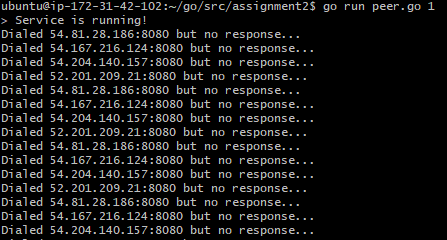
\includegraphics[width=0.75\linewidth]{launch1.png}
\caption{Launching of the first client.}
\label{fig:1}
\end{figure}

\begin{figure}[h]
\centering
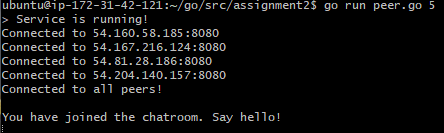
\includegraphics[width=0.75\linewidth]{launch5.png}
\caption{Launching of the last client.}
\label{fig:2}
\end{figure}

We launch the client in this order: $1, 2, 3, 4, 5$. As you can see, the first client, when launched, is the only one online so it will keep dialling other clients but will not get a response (figure \ref{fig:1}). When the last client is launched, it will be able to connect to every client that it will be looking for, therefore we see the result on figure \ref{fig:2}. 

\begin{figure}[h]
\centering
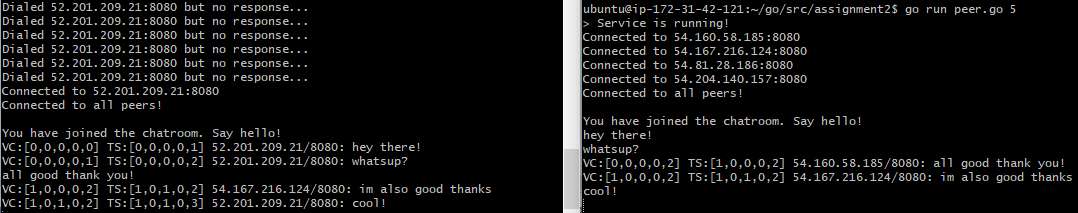
\includegraphics[width=\linewidth]{speaking.png}
\caption{Conversation of 3 clients.}
\label{fig:3}
\end{figure}

On figure \ref{fig:3} we see that first all clients are connected, then client 5 (right) says \textit{hey there!} and then \textit{whatsup?}. We see the delivery on the client 1 (left), and then this client responds \textit{all good thank you!}. Another client also joins the conversation by saying \textit{im also good thanks}, and we see the delivery of this message on both sides. Lastly, client 5 responds with \textit{cool!}. Notice that we explicitly show the vector clock and message time stamp on the delivery of a message.

\begin{figure}[h]
\centering
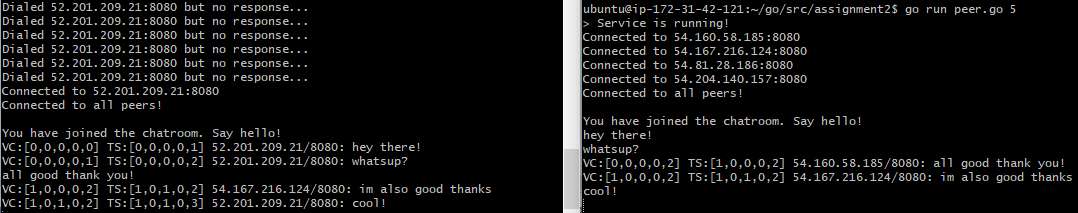
\includegraphics[width=\linewidth]{speaking.png}
\caption{Causally ordered delivery.}
\label{fig:4}
\end{figure}

On figure \ref{fig:4} we see how the causal ordering works. This is actually a continuation of figure \ref{fig:3}. We see that at client 1 (left) side, \code{\textbf{\_\_VEC\_\_}} prints the vector clock, \code{\textbf{\_\_BUF\_\_}} shows the buffer, which is empty at first time. Then, client 5 (right) sends a \code{\textbf{\_\_DELAY\_\_}} message, which is recieved but not delivered by the clients. We can see this by checking the buffer again. After that, client 5 sends a message: \text{this is after the delay} and client 1, upon recieving this, first delivers the delayed message from the buffer and then the actual message, thus showing the causally ordered delivery.

\begin{figure}[h]
\centering
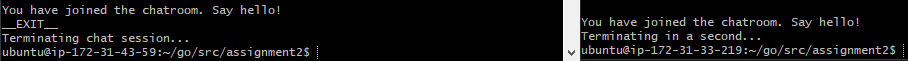
\includegraphics[width=\linewidth]{exit.png}
\caption{\textbf{\code{\_\_EXIT\_\_}} message. On the left, we see the client that sends the message. Notice how it exits immediately. On the right, we see a client that recieves that message.}
\label{fig:5}
\end{figure}

Thus we conclude that we have implemented every task given to us in the assignment. Functionalities will be demonstrated in further detail during the actual one-to-one demonstrations.

\end{document}